\documentclass[a4paper,11pt,titlepage]{article}
\usepackage[polish]{babel}
\usepackage[OT4]{fontenc}
\usepackage[utf8]{inputenc}
\usepackage{multirow}
\usepackage{graphicx} 

\author{Wojciech Żółtak (wz292583)}
\title{\emph{Opis protokołu do obsługi serwisu cytatów-sentencji}}

\frenchspacing
\begin{document}

\maketitle
% Wstawienie spisu treści:

Niniejszy dokument opisuje specyfikację protokołu do serwisu
cytatów-sentencji.

\section{Cele}
Głównym celem protokołu jest przesyłanie losowo wybranych cytatów z
bazy danych do aplikacji klienckiej.

\section{Założenia}

\begin{itemize}
\item Opisywany protokół działa w {\bf warstwie aplikacji} na zasadach
      paradygmatu {\bf klient-serwer}.
\item Umożliwia przesyłanie {\bf losowo wybranych} cytatów z bazy danych
      udostępnionej przez serwer.
\item Zakładamy działanie w środowisku, w którym działanie w ramach
      określonego okna czasowego jest istotniejsze od pewności transmisji,
      tzn. przedkłada prędkość obsługi żądania klienta nad gwarancję
      dostarczenia do niego wiadomości. Z tego powodu komunikacja będzie
      odbywać się za pośrednictwem {\bf UDP}.
\item Znakomita większość cytatów wysyłanych do klienta nie będzie zbyt
      duża (powinna zmieścić się w jednym komunikacie), co nie znaczy, że
      protokół nie będzie umożliwiał przesyłania dłuższych sentencji.
\item Serwer dysponuje bazą danych cytatów (pozostawioną w gestii
      implementacji), która pozwala jednoznacznie zidentyfikować każdy cytat
      za pomocą 4 bajtowego identyfikatora.
\end{itemize}


\section{Format komunikatów}

\subsection{Założenia}

\begin{itemize}
\item liczby zapisywane są w porządku sieciowym
\item ciągi znaków kodowane są w standardzie UTF-8, z UNIXowymi znakami końca linii, bez znaku zero na końcu
\end{itemize}

\subsection{Żądanie cytatu}

\begin{verbatim}
REQ_MSG_T {
    uint8_t type; /* := RANDOM_MSG */
}
\end{verbatim}

\begin{verbatim}
REQ_MSG_CHUNK_T {
    uint8_t  type; /* := SPECIFIC_MSG */
    uint32_t q_id;
    uint8_t  q_chunk;
}
\end{verbatim}

Opis pól:
\begin{itemize}
\item type - determinuje typ komunikatu, \texttt{RANDOM\_MSG} dla \texttt{REQ\_MSG}, \texttt{SPECIFIC\_MSG} dla
      \texttt{REQ\_MSG\_CHUNK}
\item \texttt{q\_id} - liczbowy identyfikator cytatu
\item \texttt{q\_chunk} - numer części cytatu
\end{itemize}

\subsection{Odpowiedź serwera}

\begin{verbatim}
RESP_MSG_T {
    uint32_t q_id;
    uint8_t  q_size;
    uint8_t  q_chunk;
    uint8_t  q_len;
    char     q_con[MAX_LENGTH];
}
\end{verbatim}

Opis pól:
\begin{itemize}
\item \texttt{q\_id} - liczbowy identyfikator cytatu
\item \texttt{q\_size} - rozmiar cytatu w komunikatach
\item \texttt{q\_chunk} - numer części cytatu, {\bf numerowane od 1}
\item \texttt{q\_len} - długość przesyłanego tekstu w bajtach (pola \texttt{q\_con}), nie większa niż \texttt{MAX\_LENGTH}
\item \texttt{q\_con} - treść przesyłanego cytatu (bądź jego fragment)
\end{itemize}


\section{Wymiana komunikatów}

\subsection{Założenia}
\begin{itemize}
\item Serwer działa na pojedynczym, określonym porcie, którego numer znany
      jest klientowi.
\item Klient wysyła żądania na znany port serwera, korzystając z
      dowolnego portu.
\item Serwer wysyła odpowiedź na adres nadawcy żądania, uzyskany podczas
      odbierania wiadomości.
\end{itemize}

\subsection{Stany serwera}
Serwer działa bezstanowo. W każdym momencie przyjmuje żądanie od klienta i odsyła
mu odpowiedź w postaci jednej lub więcej struktur typu \texttt{RESP\_MSG}.

\subsection{Stany klienta}

Klient może znajdować się w następujących stanach:
\begin{itemize}
\item \texttt{BEGIN} - stan wejściowy. Nie posiadamy żadnych wiadomości.

\item \texttt{REQUEST\_QUOTE} - wysyła do serwera zapytanie o losowy cytat,
w postaci struktury \texttt{REQ\_MSG} z ustawionym polem \texttt{type} na
\texttt{RANDOM\_MSG}.

\item \texttt{WAIT\_FOR\_FIRST} - oczekiwanie na pierwszą wiadomość od serwera,
w postaci dowolnej struktury \texttt{RESP\_MSG}. Jeśli otrzymana wiadomość
zawiera kompletny cytat (pole \texttt{q\_size} zawiera 1), klient przechodzi 
do stanu końcowego \texttt{END}. Jeśli wiadomość jest tylko fragmentem cytatu
(pole \texttt{q\_size} zawiera liczbę większą niż 1), klient zeruje licznik prób
i przechodzi do stanu \texttt{WAIT\_FOR\_REST}. W przypadku gdy nastąpił
\texttt{TIMEOUT}, ale nie \texttt{MAX\_TRIES}, klient ponawia prośbę wiadomość
i powraca do stanu \texttt{REQUEST\_QUOTE}. W przypadku, gdy przekroczono limit
prób i wciąż nie otrzymano wiadomości, klient przechodzi do stanu
\texttt{ABORT}.

\item \texttt{WAIT\_FOR\_REST} - oczekiwanie na pozostałe wiadomości od
serwera w postaci struktur \texttt{RESP\_MSG} zawierających takie samo
\texttt{q\_id} jak wiadomość otrzymana w stanie \texttt{REQUEST\_QUOTE}
oraz \texttt{q\_chunk} z zakresu $[1, \texttt{q\_size}]$. Jeśli klient
odbierze wiadomości dla wszystkich poprawnych \texttt{q\_chunk} przechodzi
do stanu \texttt{END}. W przypadku gdy nastąpił \texttt{TIMEOUT}, ale nie
\texttt{MAX\_TRIES}, klient stara się uzyskać brakujące części cytatu
przechodząc do stanu \texttt{REQUEST\_CHUNKS}. W przypadku gdy przekroczono
limit prób i wciąż nie uzyskano kompletu wiadomości, klient przechodzi w stan
\texttt{ABORT}.

\item \texttt{REQUEST\_CHUNKS} - wysyła do serwera zapytanie o brakujące
części w postaci struktur \texttt{REQ\_MSG\_CHUNK} (po jednej dla każdego
brakującego fragmentu) - wypełniając pole \texttt{type} na
\texttt{SPECIFIC\_MSG}, \texttt{q\_id} na wartość otrzymaną w stanie
\texttt{WAIT\_FOR\_FIRST} oraz \texttt{q\_chunk} kolejno na wszystkie
wartości, których nie otrzymano w stanie \texttt{WAIT\_FOR\_REST}. Następnie,
klient wraca do stanu \texttt{WAIT\_FOR\_REST}.

\item \texttt{ABORT} - operacja z jakichś powodów zakończyła się niepowodzeniem
i nie będzie dalszych prób jej realizacji.

\item \texttt{END} - stan wyjściowy. Klient posiada wszystkie potrzebne kawałki
cytatu, w postaci pól \texttt{q\_con}, w otrzymanych strukturach
\texttt{RESP\_MSG}, które złącza w jeden ciąg znaków według porządku po
zawartości pól \texttt{q\_chunk}.

\end{itemize}

Poniższy schemat opisuje przejścia między stanami:

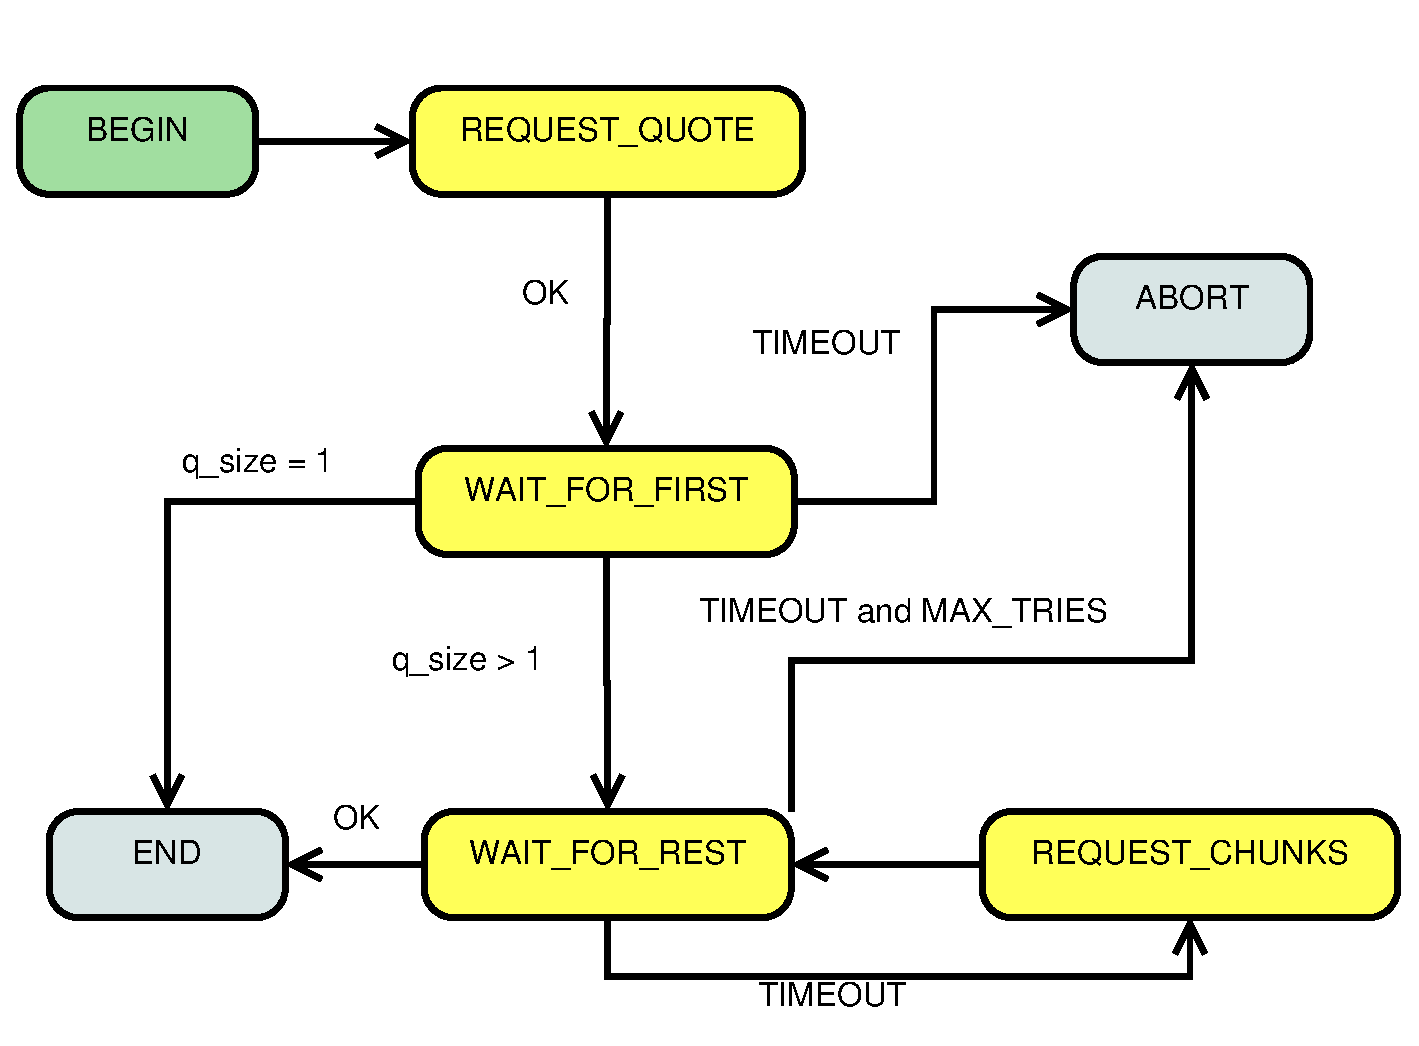
\includegraphics{klient}

\section{Używane stałe i etykiety}

\begin{itemize}
\item \texttt{RANDOM\_MSG} := 0
\item \texttt{SPECIFIC\_MSG} := 1
\item \texttt{MAX\_LENGTH} - maksymalna długość tekstu przesyłanego w jednym komunikacie;
protokół nie wymusza konkretnej wartości, lecz sugerowane są nie za duże
liczby (w okolicach 1000, np. 1018 octetów, tak żeby cały komunikat miał
ich 1024)
\item \texttt{TIMEOUT} - zdarzenie przekroczenia limitu oczekiwania na odpowiedź serwera;
długość oczekiwania w gestii implementacji
\item \texttt{MAX TRIES} - zdarzenie przekroczenia ilości prób pobierania brakujących fragmentów wiadomości;
ilość prób w gestii implementacji, może być różna dla różnych stanów (np. stan 
\texttt{WAIT\_FOR\_REST} może pozwalać na większą ilość prób, niż
\texttt{WAIT\_FOR\_FIRST})
\end{itemize}

\end{document}
